\subsection{Калибровка точного времени (Fine time calibration)}\label{section:FTcalib}

Пример таблицы калибровки точного времени, полученной на данных лабораторных тестов, представлен в виде графика на рисунке \ref{fig:TypicalCalibTable}. По оси абсцисс откладывается значение счётчика точного времени, а по оси ординат --- значение точного времени в наносекундах. Вид графика не зависит от того, по каким данным он был построен, так как он определяется архитектурой время-цифрового преобразователя. Обратим внимание, что в диапазоне значений десятибитного счетчика точного времени интервалу равному периоду грубого счетчика, т.е. 5~нс, соответствуют отсчеты от 30 до 520. Точные границы интервала определяются тем, что значения задержек отдельных элементов цифровой линии задержки индивидуальны и зависят от флуктуаций технологического процесса.
%Было: Точные границы интервала определяются тем, что задержки на каждой ступени индивидуальны и зависят от флуктуаций технологического процесса.
% хотя бы - на каждом элементе

С целью понимания особенностей работы счетчиков точного времени, каждая таблица калибровки точного времени была фитирована кусочно-линейной функцией. На рисунке \ref{fig:CalibTableMinusFit} показан пример разности значений функции калибровки точного времени и линейной функции. Видно, что отклонения не превышают 60 пс.
% фитирована - аппроксимирована

% Макросы для получения этих картинок лежат в Data_analysis_repo/threshold_scan_2/
\begin{figure}
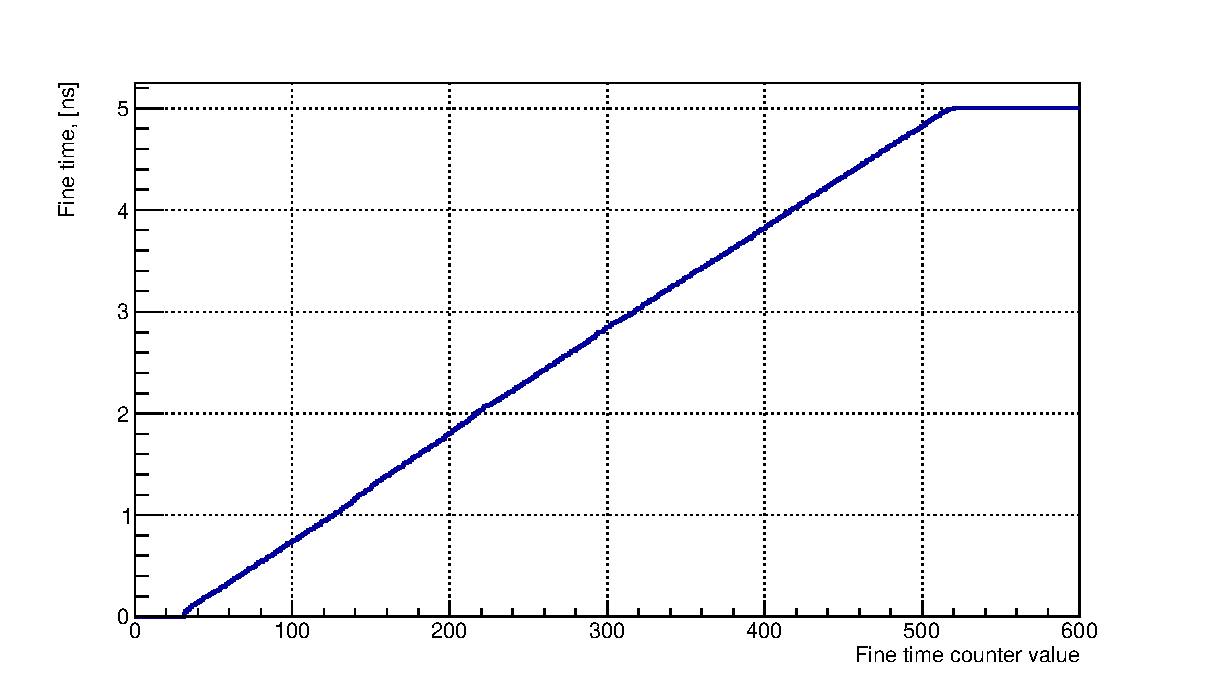
\includegraphics[width=1.0\textwidth]{pictures/CalTable_0010_01.eps}
\caption{Пример калибровочной кривой.}
\label{fig:TypicalCalibTable}
\end{figure}

% Макросы для получения этих картинок лежат в Data_analysis_repo/threshold_scan_2/
\begin{figure}
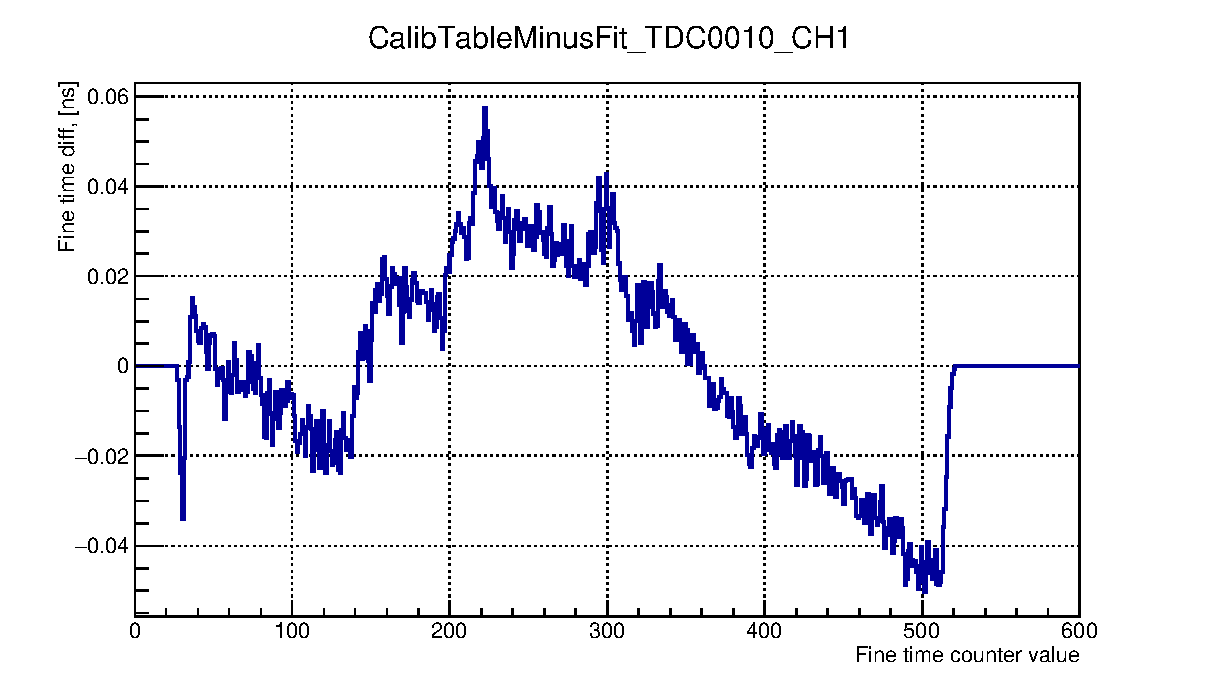
\includegraphics[width=1.0\textwidth]{pictures/CalTableMinusFit_0010_01.eps}
\caption{Отклонение калибровочной кривой от линейной функции.}
\label{fig:CalibTableMinusFit}
\end{figure}

Каждая аппроксимирующая кусочно-линейная функция состоит из трёх отрезков и может быть однозначно описана двумя координатами изломов, которые приблизительно соответствуют двум крайним рабочим значениям счётчика точного времени. Параметры линейных функций для всех каналов отображены на двумерной гистограмме на рисунке \ref{fig:ABmap}.
% строго говоря, это не гистограмма (диаграмма?)
Видно, что распределение хотя и двугорбое, но достаточно компактное.

Один из возможных способов оценки влияния калибровки на точность регистрации временных отметок это исследование физически одновременных фронтов, которые можно получить, например, с помощью высокоточного генератора прямоугольных импульсов.

%Влияние замены точной функции калибровки на приближенную можно увидеть при одновременной оцифровке на нескольких каналах ВЦП сигналов с высокоточного генератора прямоугольных импульсов.
%(Сначала нужно сказать, что для оценки качества калибровки необходимо исследовать одновременные фронты, которые можно получить от высокоточного генератора прямоугольных импульсов.)
%(Расписать подробно ряд: точная калибр., индивид. линейная функция, глоб линейная функция, отсутствии калибр.)

В процедуре калибровки для каждого канала была выполнена замена калибровочной таблицы сначала индивидуальной линейной функцией данного канала, а потом усредненной. Полученные распределения измеренной ширины импульса в исследуемом канале показаны на рисунке \ref{fig:FourToT}.

% Значение 30 пс я получил из распределения по передним фронтам, FWHM в линейной шкале. Это среднее знечение по нескольким каналам. Разброс очень маленький.
% При использовании индивидуальной калибровки получается 70 пс.
% А вот сравнивать это со случаями без калибровки или с усреднённой калибровкой не очень корретно, потому что вид распределения двухпиковый и ширина одного пика лишь немного больше, но воторой пик оказывает своё влияние.
Видно, что полноценная калибровка точного времени необходима для достижения предельной точности ВЦП, составляющей 30~пс (FWHM). Использование индивидуальной линейной функции приводит к падению точности до 70~пс, а усреднённой --- до ??? (без калибровки) в наиболее неблагоприятных каналах.
Таким образом, при невозможности выполнить калибровку точного времени, например, из-за недостаточного массива данных, предоставленных для анализа, в условиях нашей задачи, когда характерное временное разрешение составляет несколько сотен пикосекунд, возможно применение усредненной линейной функции без заметного снижения точности.

% Макросы для получения этих картинок лежат в Analysis_Sep2016/WLS_off/calibration_files/
\begin{figure}
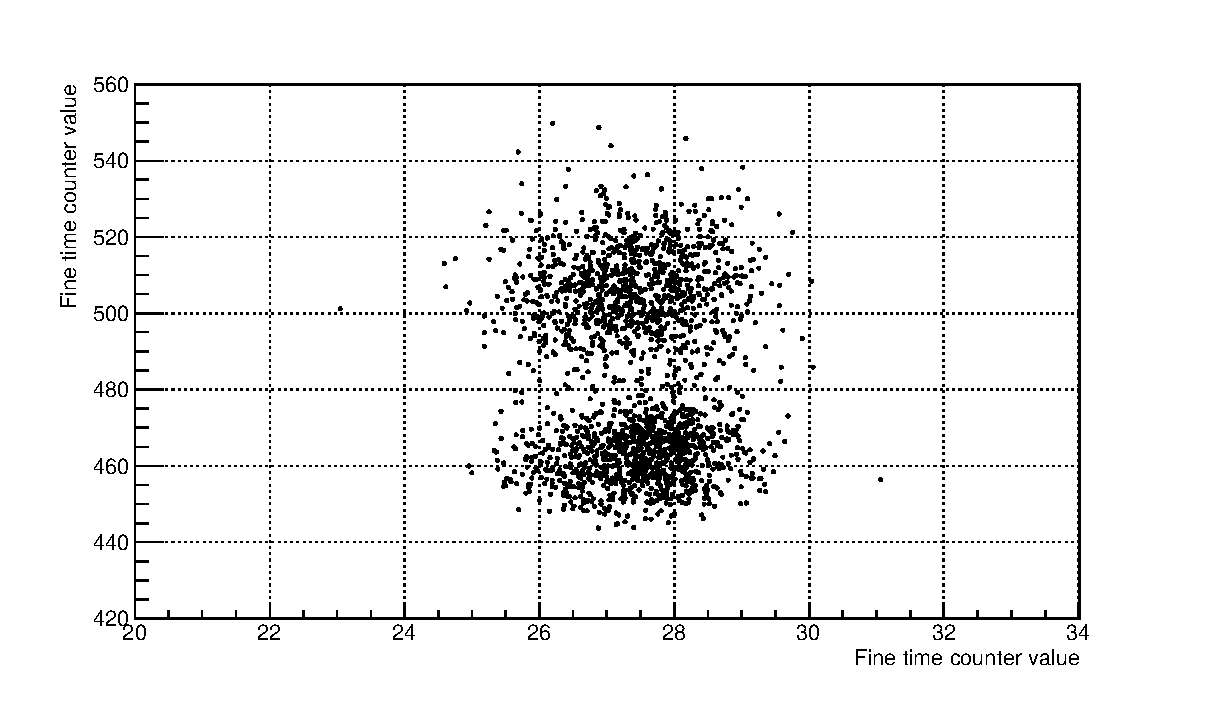
\includegraphics[width=1.0\textwidth]{pictures/ABmap.eps}
\caption{Распределение координат точек излома аппроксимирующих кусочно-линейных функций.}
% для большого набора каналов по данным с пучковых тестов
\label{fig:ABmap}
\end{figure}

% Макросы для получения этих картинок лежат в Data_analysis_repo/directTDC/
\begin{figure}
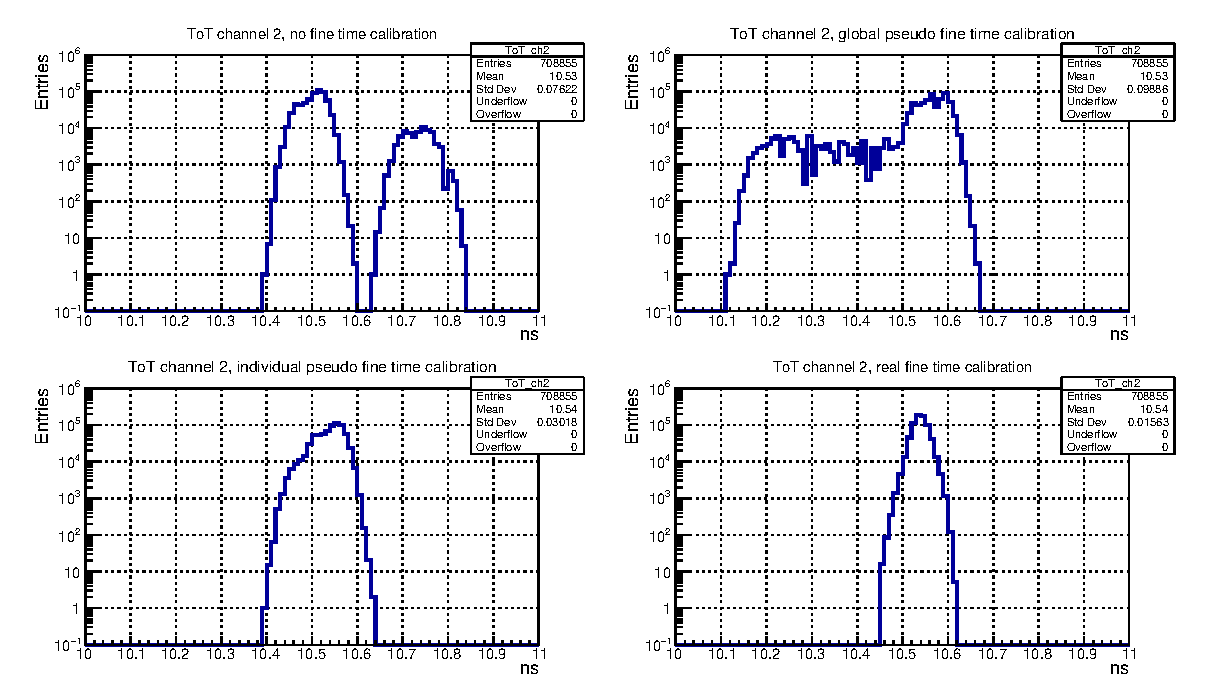
\includegraphics[width=1.0\textwidth]{pictures/ToT_ch2.eps}
\caption{Результаты измерения ширины импульса от генератора в случае: без калибровки точного времени; с применением усреднённой калибровочной фукнции; с применением индивидуальной линейной калибровочной функции; с применением полноценной калибровочной таблицы.}
\label{fig:FourToT}
\end{figure}

Приведённые выше функции калибровки были построены по массиву данных, содержащихся в семи файлах. Каждый файл это 2~минуты измерений при частоте генератора 5~кГц, т. е. около 600~тысяч вспышек лазера. Таким образом, всего было 4.2~миллиона вспышек за  14~минут, а один файл составляет приблизительно 15\%~от полного набора данных. В каждом канале было зарегистрировано от~300 до~400~тысяч временных отметок, которые были использованы для выполнения калибровки. Для иллюстрации стабильности калибровки на рисунке~\ref{fig:Stability} показана разность функций калибровки, построенных по всему массиву данных и функций, построенных на файлах, составляющих $ \approx $15\%~данных каждый, взятых в начале, середине и конце набора данных. Видно, что отклонения в основном не превышают 10~пс, однако имеются редкие выбросы до 20~пс.

\begin{figure}
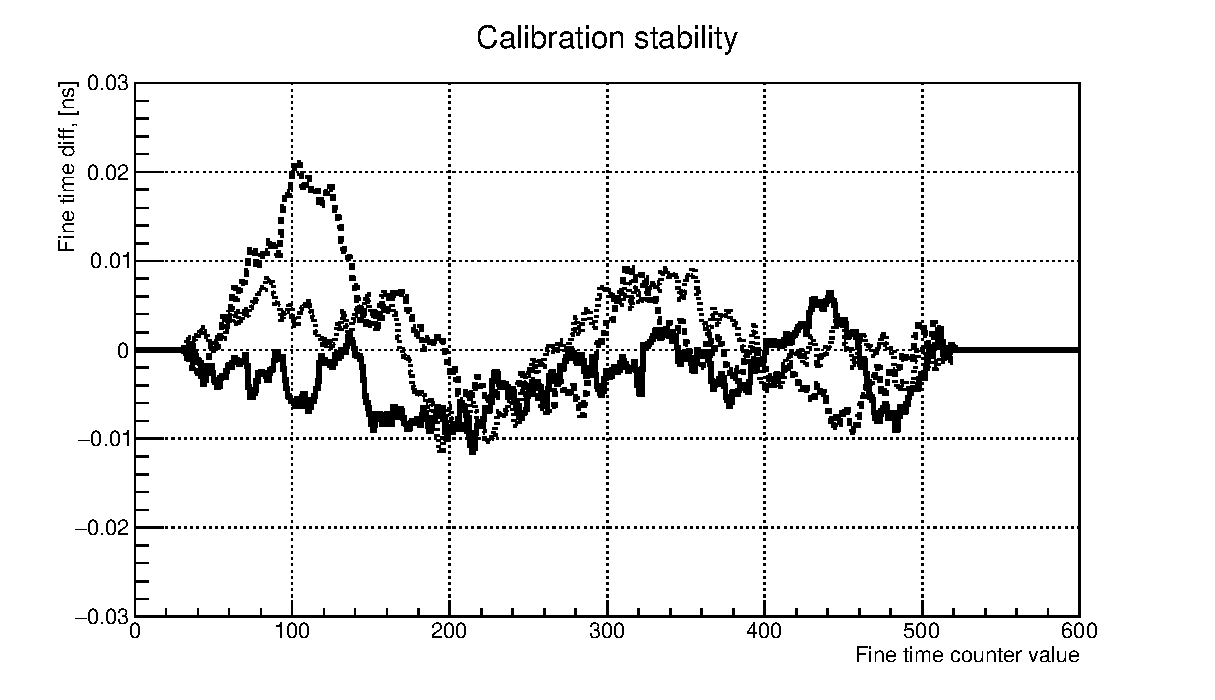
\includegraphics[width=1.0\textwidth]{pictures/calibrationStability_dec2016.eps}
\caption{Стабильность калибровок.}
\label{fig:Stability}
\end{figure}
